Library generation is the process of creating of a large set of primitives $P$, each of which define a trajectory $\Phi(\theta^+) \to \Phi(\theta^-)$, where $\Phi(\theta^+), \Phi(\theta^-) \in \tilde{Q}$, the set of all impact configurations. The library is intended to be structured such that efficient on-line use is enabled. Minimising off-line computation time is a secondary concern.

\subsection{Acceptable coverage}
As motivated in the previous section, a useful library of motion primitives for walking over uneven terrain requires coverage over the start and final configurations of the robot along with a range of kinetic energy additions and subtractions. Depending on the unevenness of the terrain, a diverse range of paths of the end of the swing leg may also be required. All generated constraints should be admissible and usable to avoid wasted memory and computation time.

While it is clear that some density of coverage is required, it is not immediately obvious what constitutes sufficiency. It is advantageous to avoid over-populating the library in order to speed up its generation and real-time use and reduce the memory requirements. However, advantages in computation time are meaningless if the library is insufficient for its purpose. As a result, methods for defining acceptable coverage of the dimensions of this optimisation are required.

\subsubsection{Start and end configurations}
It is essential that the library is designed such that final configurations of virtual constraints match initial configurations of other constraints through the impact map. A primitive is not useful if there are no primitives which can succeed it. Other than a detailed study of the terrain on which the robot is intended to be used, there is no good means for deciding on sets of configurations which should be reachable through a single constraint from a given configuration, therefore it seems necessary to generate a set of virtual constraints linking each pair in $\tilde{Q}\times\tilde{Q}$. This provides further motivation to avoid specifying more impact configurations than necessary, since the number of virtual constraints in the library $\lvert P \rvert \propto \lvert\tilde{Q}\rvert^2$.

The most important consideration for impact configuration coverage is to ensure that there is a relatively fine grid of vertical displacements $p_v(\theta^-)$ for a given horizontal displacement to allow for the traversal of the robot over unpredictable terrain. The resolution and bounds of this grid should chosen be such that the intended terrain is properly discretised; large gaps between the upper/lower bounds and the maximum displacement of the expected terrain should be avoided. Certainly, the upper and lower bounds should not exceed the capability of the robot. Furthermore, the resolution should be comparable in size to the combined error in the robot's perception of the terrain and the closeness to which the controller can regulate a trajectory. As is evident from these requirements, the best choice of grid for height values depends on the terrain and robot for which the library is being designed. We denote the number of unique step heights $n_y$.

It is much less important to have a dense grid of horizontal displacements. Indeed, dynamic walking over uneven terrain in most instances achievable with a fixed step length. This fact forms the basis of much of the previous work using feedback-stabilised periodic gaits to enable locomotion over relatively uneven terrain \cite{bigdog?}. Having a set of step lengths is advantageous in that it enables for intelligent foot placement. Denote the number of unique step lengths $n_x$.

Other than in the case of the compass-gait robot, the step length and height are not sufficient to specify the final configuration of the robot. It is therefore necessary to perform inverse kinematics to generate joint angles. In the general case, there are infinitely many combinations of joint angles which can produce the final configuration for a particular step length and height. There is no general method for producing the best configuration; it depends on the robot's mechanical design and the desired gait. While not strictly necessary for terrain scalability, the energy efficiency of planned trajectories can be improved by having multiple configurations of joints per step length and height from which to choose. Let us denote the number of these configurations $n_q$.

The cardinality of the set of all impact configurations is trivially evaluable:
\begin{equation} \label{eqn:numimpactconfs}
\lvert\tilde{Q}\rvert = n_xn_yn_q
\end{equation}
We note that while $n_q$ must be fairly large to enable walking over uneven terrain, $n_x$ and $n_q$ are useful only to provide additional control and should be kept small. Under Equation \ref{eqn:numimpactconfs}, $\lvert P \rvert \propto \lvert\tilde{Q}\rvert^2 \implies \lvert P \rvert \propto n_x^2 ~~\wedge~~ \lvert P \rvert \propto n_q^2$.

\subsubsection{Inter-step kinetic energy changes}
The only method of velocity control available to the motion planner is to chose constraints which add, maintain or reduce the kinetic energy of the walker. It is therefore important to produce, for each pair of step length and height, a range of kinetic energy mutations. For simplicity, we produce a set of kinetic energy additions and subtractions $\tilde{K}$, where $\lvert\tilde{K}\rvert = n_k$. For each set of initial and final configurations $q^+,q^- \in \tilde{Q}$, we produce the $n_k$ unique trajectories $q^+ \to q^-$ with $\Delta$KE $\in \tilde{K}$.

For a given robot, it may be possible to define a particular range of $\Delta$KE values on the basis of the initial and final configuration. For instance, since a step-up trajectory converts kinetic into potential energy, constraints which add the maximum kinetic energy may not ever be chosen by the motion planning algorithm. Such reasoning is difficult to properly justify in general and as such has not been pursued in this thesis work. Even if such reasoning is used, it is still likely best to produce $n_k$ paths.

We need not be as strict on keeping $n_k$ small, since $\lvert P \rvert \propto n_k$ rather than $n_k^2$, however since velocity control is able to be executed over multiple footsteps, the precision and variety of $\Delta$KE over a single footstep is not critical. Therefore in the interest of keeping the library manageable, $n_k$ should be kept to a moderate size.

Note that while the initial and final configurations are important data for a virtual constraint, the target $\Delta$KE should not be stored. As discussed previously, the change in kinetic energy is dependent on the initial velocity of the constraint. Furthermore, its calculation requires very little computation due to the affine form of the partial solution.

\subsubsection{Ground configurations}
It is important to consider the likely shape of the ground for constraints with particular step lengths and heights. For the off-line generation of virtual constraints, it is best to be somewhat conservative in specifying where the ground level changes. Consider Figure \ref{fig:stepup}; the terrain steps up at a horizontal displacement significantly smaller than $p_h(\theta^-)$. It is reasonable to expect that this is representative of the typical use case of a step-up virtual constraint. It is not necessary to optimise numerous primitives with all else fixed but with varied ground configurations; if the terrain profile for the purposes of each single VC optimisation is conservatively defined, the ground configuration is indirectly sampled by producing constraints with varying initial and final configurations.

\begin{figure}
	\centering
	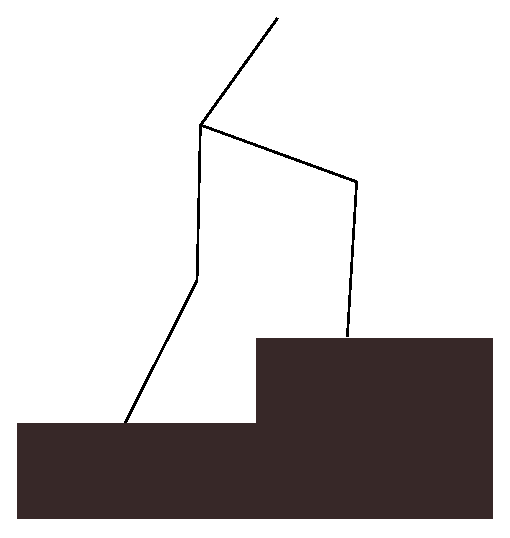
\includegraphics[width=0.5\linewidth]{4VirtConstLib/stepup.eps}
	\caption{Example step-up showing possible terrain profile}
	\label{fig:stepup}
\end{figure}

\subsection{Ordering sets of constraints} \label{sec:orderings}
As discussed in Section \ref{sec:primplanning}, planning with primitives is made much more efficient if there is an ordering of primitives, since this facilitates a binary search, reducing the worst-case search time from $O(n)$ to $O(\log n)$. Ordering on the basis of $\Gamma(\theta^\bullet)$ and $\Psi(\theta^\bullet)$

\subsection{Library structure}
The structure of the library is a critical issue in determining the running time of the planning algorithm. It is important that constraints with certain properties can be found efficiently and that traversal through the library is straightforward. The library of motion primitives, as pictured in Figure \ref{fig:lib} is structured similarly to that described in \cite{manchester13planning}.

\begin{figure}
	\centering
	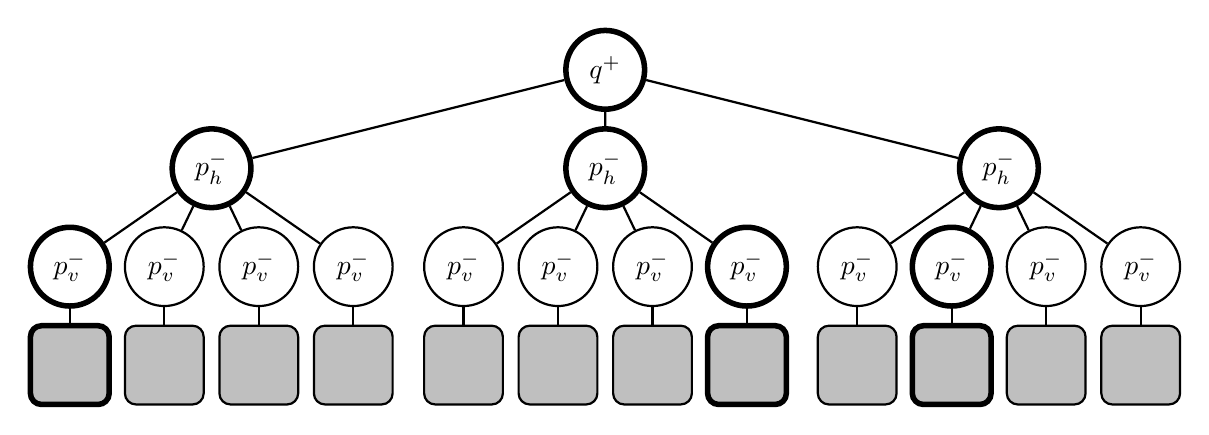
\begin{tikzpicture}[
	scale = 1, transform shape, thick,
	every node/.style = {draw, circle, minimum size = 10mm},
	grow = down,  % alignment of characters
	level 1/.style = {sibling distance=5cm},
	level 2/.style = {sibling distance=1.2cm}, 
	level 3/.style = {sibling distance=1.2cm}, 
	emph/.style={edge from parent/.style={red,very thick,draw}, line width = 2pt},
	norm/.style={edge from parent/.style={black,thin,draw}},
	leaf/.style={shape = rectangle, rounded corners, fill = gray!50},
	level distance = 1.25cm
	]
	
	\begin{scope}[xshift=0cm]
	\node[emph] {$q^+$} 
	child { node [emph] {$p_h^-$}
		child {   node [emph] {$p_v^-$}
			child { node [leaf,emph]  {}}
		}
		child {   node [norm] {$p_v^-$}
			child { node [leaf]  {}}
		}
		child {   node [] {$p_v^-$}
			child { node [leaf]  {}}
		}
		child {   node [] {$p_v^-$}
			child { node [leaf]  {}}
		}
	}
	child { node[emph] {$p_h^-$}
		child {   node [] {$p_v^-$}
			child { node [leaf]  {}}
		}
		child {   node [] {$p_v^-$}
			child { node [leaf]  {}}
		}
		child {   node [] {$p_v^-$}
			child { node [leaf]  {}}
		}
		child {   node [emph] {$p_v^-$}
			child { node [leaf,emph]  {}}
		}
	}
	child { node[emph] {$p_h^-$}
		child {   node [] {$p_v^-$}
			child { node [leaf]  {}}
		}
		child {   node [emph]{$p_v^-$}
			child { node [leaf,emph]  {}}
		}
		child {   node [] {$p_v^-$}
			child { node [leaf]  {}}
		}
		child {   node [] {$p_v^-$}
			child { node [leaf]  {}}
		}
	};
	\end{scope}
	\end{tikzpicture}
	\caption[Virtual constraint library structure]{Virtual constraint library structure. Each leaf contains $n_qn_k$ primitives in a sorted array. A possible (worst-case) search path is indicated in bold. Note that only  one initial condition $q^+\in\tilde{Q}$ is pictured. The library contains many repetitions of this structure.}
	\label{fig:lib}
\end{figure}

The library is built using a hierarchical (forest) structure with each of the impact configurations in $\tilde{Q}$ at the top. Consider this the initial configuration of the robot. Connected to each root node are $n_x$ nodes representing a particular step length $p_h(\theta^-)$. To each of these nodes are connected $n_y$ edges, encoding the grid of step heights $p_v(\theta^-)$. These edges are sorted in ascending order of height. At each of the nodes reachable from these edges, we have an encoded step length and height. This is important since there is only one height for a given length which is applicable based on the terrain.

Each of these nodes is associated with a sorted array containing $n_qn_k$ applicable trajectories $q^+ \to q^-$, specified by Bézier coefficients as discussed in Section \ref{sec:bezconstraints}. These paths are able to be sorted based upon the ordering method introduced in Section \ref{sec:orderings}. The library is therefore conducive to an efficient search from a particular initial configuration $q^+$ to a trajectory $q^+ \to q^-$ on the basis of first matching step heights to the terrain at given step lengths, then searching through only the applicable constraints for a desired velocity or kinetic energy. Note that since the primitives are ordered, this search is completed in $\mathcal{O}(n_x\log(n_yn_qn_k))$ time. This is clearly preferable to the $\mathcal{O}(n_xn_yn_qn_k)$ time of a search through an unstructured array of all primitives in $P$. We may again motivate the need to keep $n_x$ small; the worst-case search time is logarithmic in $n_y$, $n_q$ and $n_k$ but linear in $n_x$.

\subsection{Library generation implementation}
Implemented in matlab -- a ``real'' implementation should be in a language with pointers like C.

Generation of set of impact configurations

Enforcement of condition 3-5?

Ground definition

Low-level structure - array with pointers (indexes)

Multiple orderings?